\documentclass[DIV=current]{scrartcl}

\usepackage[style=ieee]{biblatex}
\usepackage{comment}
\usepackage{graphicx}
\usepackage{subcaption}
\usepackage[urlcolor=blue,colorlinks=true]{hyperref}
\usepackage[outputdir=./build]{minted}
\usepackage{wrapfig}

% Bibliography
\bibliography{Report}

% Title Header
\titlehead{SWE30011 \hfill Alastair Knowles \\ \parbox{\textwidth}{\hfill 2062674}}

% Rather than using builting BCOR or DIV (look at docs), we are setting the area explicitly
% to give us more room for code. This spits out annoying warnings though (so probably not the
% "proper" way of doing things)
%\areaset{0.85\paperwidth}{0.85\paperheight}

% Settup minted files here

\newmintedfile[includecpp]{cpp}{linenos=true,fontsize=\scriptsize,breaklines=true,tabsize=4}
\newmintedfile[includepy]{python}{linenos=true,fontsize=\footnotesize,breaklines=true,tabsize=4}
\newmintedfile[includehtjin]{html+jinja}{linenos=true,fontsize=\footnotesize,breaklines=true,tabsize=4}
	
\title{A vehicle monitoring proof of concept}
\subtitle{%
	\vspace{0.5em}
	\textmd{%
		\begin{tabular}{lr}
			Lab Session & Friday 14:30 \\
			Tutor  & Harindu Korala
		\end{tabular}
	}
}
\author{\vspace{-1em}}
\date{\vspace{-3em}}

\begin{document}

	\maketitle
	
	% 1. 10% - Introduction of your application and its components
	% 2. 10% - IoT hardware details and description including the technical information
	% 3. 10% - Software implementation details including the description of the codes
	% 4. 10% - Data Management – Including the implementation and design of the data model, database and data communications
	% 5. 10% - Description and details of the APIs and Webservers you are using
	% 6. 10% - IoT Networking – details of the potential IoT network including the motivation for choosing the protocol and network diagram
	% 7.  5% - IoT Cloud computing – Potential cloud computing techniques for your IoT application
	% 8.  5% - Potential Machine Learning and Advanced Data Analytics techniques that can be added to your IoT project
	% 9.  5% - IoT Security challenges and solutions for your IoT project
	% 10. 5% - Challenges, Limitations, and future work
	
	
	\section{Introduction}
	Within the vehicle industry, there has been a big push to integrate technology within up and coming vehicles. Introducing technologies such as vehicle GPS tracking, autonomous driving and remote vehicle monitoring. Much of this technology is generally only available in high end vehicles, with no real solution for older cars and trucks. Being able to install such a system within older vehicles would be advantageous, as it significantly reduces the price barrier for these technologies, and is a fantastic interim solution for low income households, particularly because the statistics may allow them to save money over time.
	
	% System with multiple sensors
	% - OBD2 monitor - didnt get time. also least ``IoT Node'' like device of all.
	% - GPS module - Current position. Online truck tracking. Delivery statistics
	% - MEMS module - Bearing, hills vs fuel analysis, additional sensory data for future deep analysis
	% - Future: Human monitoring camera - Deep learning driver fatigue analysis.
	% - Future: Route planner device - Show the driver a pre-designated route for whatever deliviery is in their truck. Routes could be pre-calculated in the cloud and integrated with the warehouse ERP system.
	
	\section{Theoretical system overview}
	There are a number of important considerations that need to be taken into account when designing a system for pre-existing vehicles. Considerations such as year of vehicle manufacture and the type of vehicle, will severely impact the overall design of nodes and edge devices. For example, OBD2 may not be available on older vehicles, as well as vehicle complexity and engine noise. Additionally, individuals may not wish to make significant wiring modifications to their car.
	
	\subsection{Hardware requirements}
	Hardware of the system is broken down into 2 main components; the edge device and nodes. Nodes will perform a myriad of sensing activities, including GPS location, acceleration, change in direction (gyroscope), absolute direction (magnetometer) and vehicle engine statistics. Edge devices will coalesce data into an easily consumable format for the cloud, which would include data analysis and transformation of information into other formats.
	
	At this stage, any embedded Linux platform may be used as an edge device, provided it has some form of bluetooth BLE communications. Future expansions may include AI vision based tiredness detection for the driver, which would require specialised hardware for Neural Network convolution, such as the Intel Myriad range of VPU chips \cite{_intel_}. For our prototype hardware, we are using a Raspberry Pi model 3B+, which has the required Bluetooth BLE built in.
	
	In a vehicle, there is an abundance of data that could be collected, including vehicle engine statistics, for determining engine health and fuel consumption, current vehicle location and routes travelled, driver tiredness, etc. For our example nodes, we chose to develop both a GPS node and an IMU node. An engine monitoring node was also planned, but acquisition of an OBD2 reader chip was not practical within the time period given.
	
	Fritzing designs for prototype GPS and IMU nodes can be seen in Figure~\ref{fig:gps-node} and Figure~\ref{fig:imu-node} respectively. Lithium Ion batteries were used for power, and breadboard used for construction. The GPS node uses an ESP32 chip as a combined microprocessor and BLE communications module. As a note, the GPS module pictured is not the same as what was used in construction. The prototype node uses a custom GPS module acquired from a past workplace with a Global Top GPS receiver module. The IMU node uses an Arduino Nano combined with a Bluetooth BLE module\cite{_arduino_} and a Sparkfun MPU-9250 module\cite{_mpu9250_}. Construction of the node devices can be seen in Figure \ref{fig:hwpic}.
	
	\begin{figure}[t]
		\centering
		\begin{subfigure}{0.54\linewidth}
			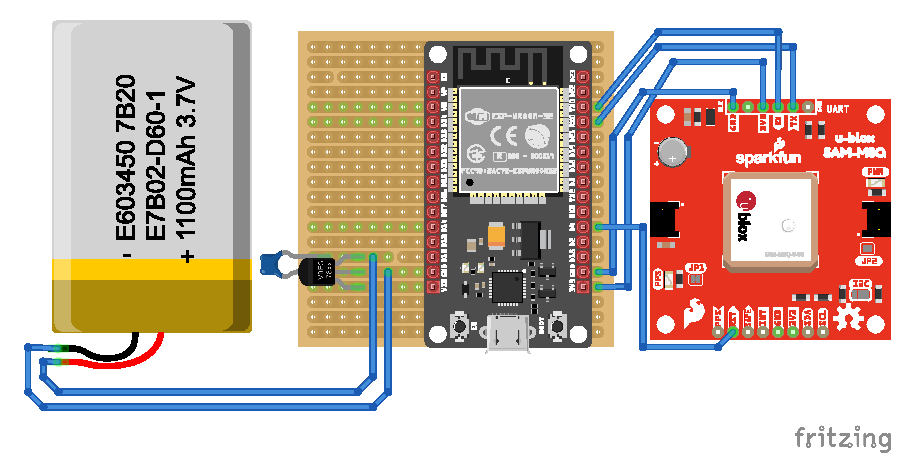
\includegraphics[width=\linewidth]{images/esp-node.pdf}
			\caption{ESP32 GPS node}
			\label{fig:gps-node}
		\end{subfigure}
		\begin{subfigure}{0.45\linewidth}
			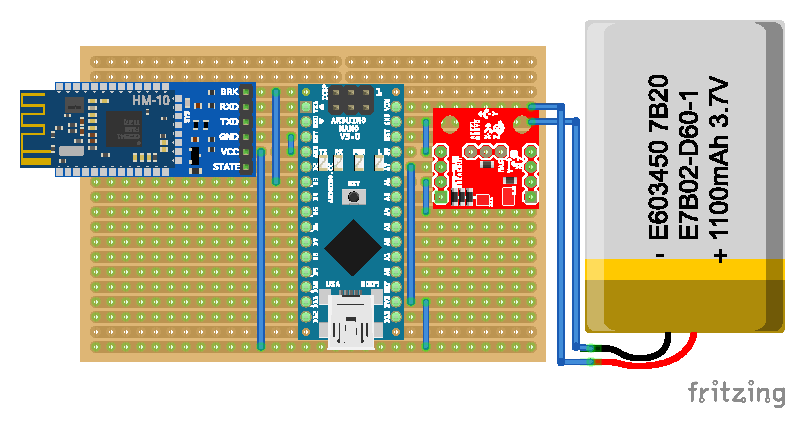
\includegraphics[width=\linewidth]{images/nano-node.pdf}
			\caption{Arduino Nano IMU node}
			\label{fig:imu-node}
		\end{subfigure}
		\caption{Node devices}
	\end{figure}
	
	\subsection{Device Communications}
	As previously stated, communications between nodes and the edge is via Bluetooth BLE. This was due to high availability of hardware, and very low cost. There are several other viable wireless communications technologies, including ZigBee, LoRaWAN and WiMax. Moving forward from the proof of concept phase to product prototypes, these wireless technologies should be considered. Additionally, CAN BUS would be a practical solution for wired communications within vehicles due to its abundance in modern cars.
	
	
	\begin{wrapfigure}{R}{0.5\linewidth}
		\centering
		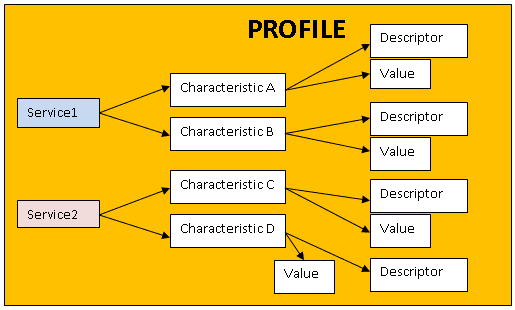
\includegraphics[width=\linewidth]{images/ble-profile.png}
		\caption{GATT attribute hierarchy}
		\label{fig:gatt}
	\end{wrapfigure}
	
	The structure of Bluetooth BLE is fundamentally different to past Bluetooth standards. Communications is structured as a hierarchy of attributes as shown in Figure \ref{fig:gatt}. At the top most level, way with A custom UART like GATT protocol was implemented on the GPS node. This included both a TX and an RX characteristic within a UART style service.
	
	Physical communication between an edge device and the cloud requires some sort of cellular connectivity, such as a 3G or 4G modem. The edge device pushes all data to the cloud via MQTT. During the proof of concept phase, a wirelessly tethered phone was used for cellular communications.
	
	\begin{figure}[h]
		\centering
		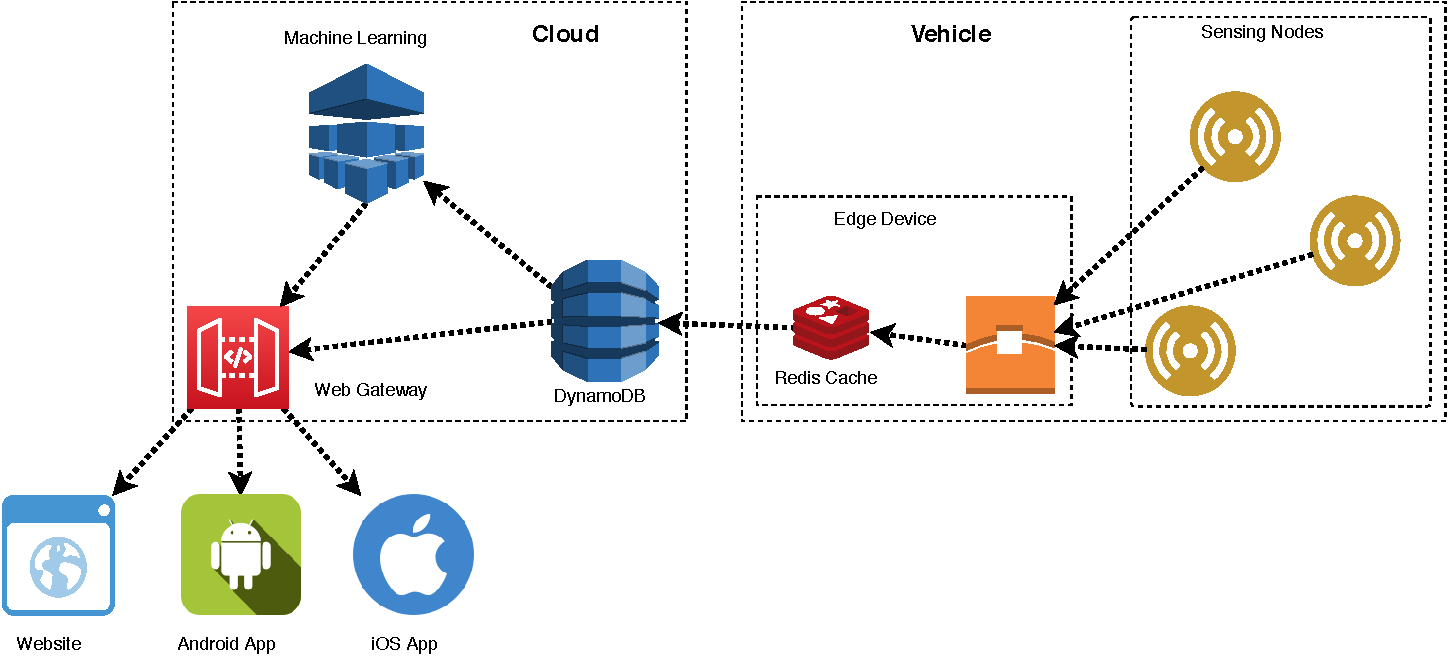
\includegraphics[width=\linewidth]{images/IoT-Diagram.pdf}
		\caption{IoT Structure overview}
		\label{fig:commsgraph}
	\end{figure}
	
	\subsection{Software}
	Node software is written in a subset of C++ called the Arduino Programming Language. The IMU node makes heavy use of the library included with the MPU-9250, which is used for fetching data via I2C. Data is then written out via the serial port to the attached bluetooth module, where it is transferred to an edge device using the Nordic UART service specification for BLE. The GPS node receives data from the onboard GPS module, which is then similarly transferred via BLE to an edge device, however the GATT service used is a custom UART like service.
	
	Software on the edge device is written in python, allowing for a rapid development of the system as a whole, and is split such that there are 2 separate programs with distinct functionality.
	
	The first program, \mintinline{bash}{gatt_manager.py}, deals with node communication via BLE. When a node comes into range, \mintinline{bash}{gatt_manager.py} connects to the device and registers for notifications. When a notification is received, data is read from the node and transformed into a digestible format for the cloud. This data is then saved to a local Redis cache for later transfer. At this stage, only GPS GATT communication are implemented.
	
	The second program, \mintinline{bash}{mqtt_manager.py}, handles communication between the edge device and the cloud. Data is pulled from the local Redis cache, and pushed to an Amazon DynamoDB instance in the cloud via mqtt. The code is fairly trivial, but the idea of first caching data within a Redis server is crucial, as it allows the edge device to intermittently disconnect without losing information.
	
	\begin{figure}[h]
		\centering
		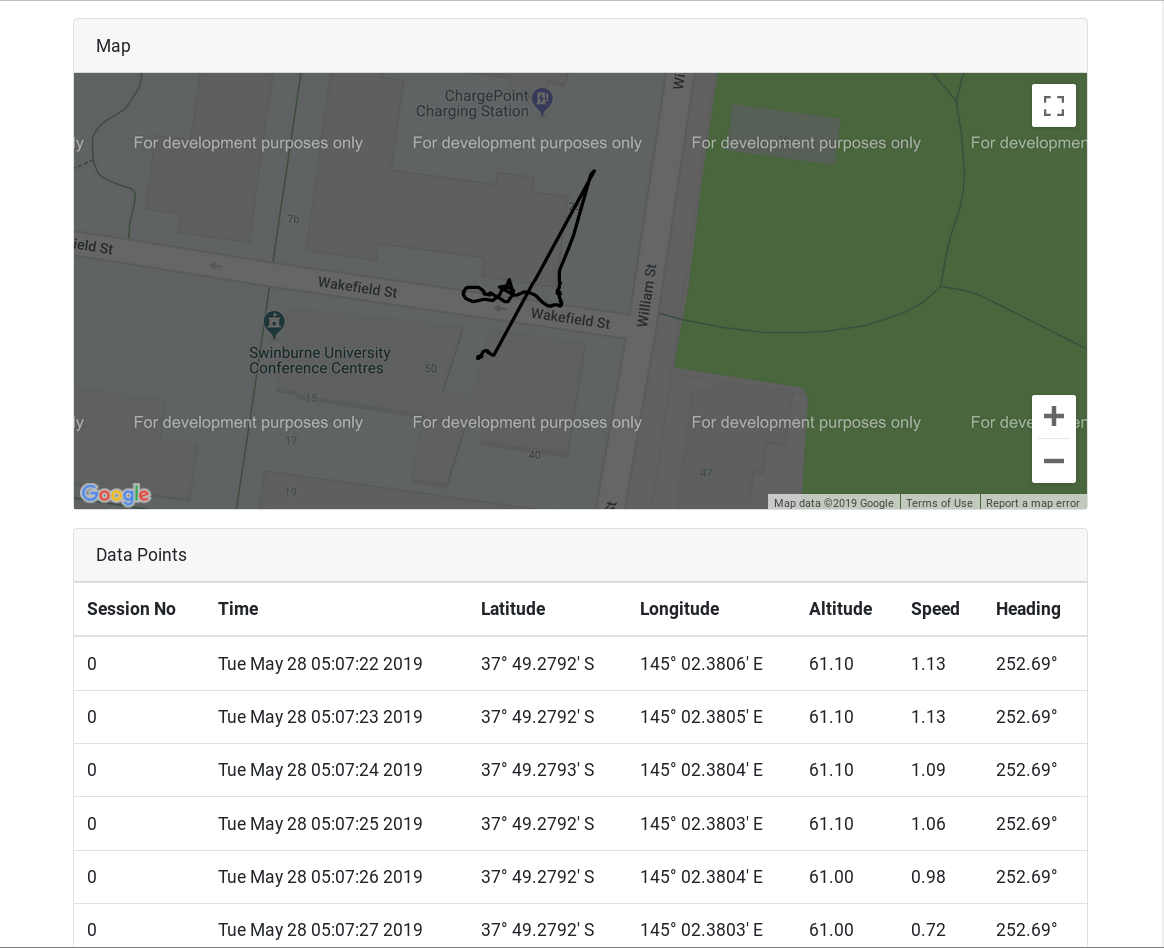
\includegraphics[width=\linewidth]{images/webpage.png}
		\caption{A simple webpage, demonstrating how data can be pulled from DynamoDB and embedded onto a map}
		\label{fig:website}
	\end{figure}
	
	Once in the cloud, data may be used in a number of different ways. Machine learning may be applied to data to detect serious problems with a vehicle, or its driver. Additionally, data may be pulled by web clients and mobile device apps. Currently, there is a simple web interface for showing GPS data on a map. Data is pulled from DynamoDB and formatted into a table, as well as displayed on a google maps instance. A screenshot of the website may be seen in Figure \ref{fig:website}.
	
	\subsection{APIs and Webservers}
	A number of different APIs are used within the proof of concept design. At the lowest level, the IMU node utilises the Sparkfun MPU-9250 library for communications with the IMU breakout board of the same name, and the GPS node uses the built-in BLE API for setup and operation of the Bluetooth BLE interface.
	
	The edge device utilises a Bluez API for communicating with the Linux Bluez bluetooth stack via DBus. DBus is a fairly modern Linux IPC mechanism, used for managing many system resources. The python-redis API is used for communicating with the internally hosted Redis database. And finaly paho-mqtt is an MQTT API used for pushing data to the cloud.
	
	The website is constructed using Flask, which was a conscious choice based on prior experience and it having been introduced within this unit as a preferred option for building websites. Data is pulled from Amazon DynamoDB using the boto3 API. And finally, Google's Google Maps API was used for displaying GPS location data on a map on the website.
	
	\subsection{Data Management}
	Within our theoretical system, data management is split into 2 stages. A local cache on the edge device (a Redis database) is used in case of cellular connectivity issues. When travelling, vehicles will often be out of range of cellular connectivity, hence a local cache is crucial.
	
	From here, data is transmitted to the cloud via MQTT. The cloud allows convenient storage of vast amounts of data for future analysis, and easy access for connected clients. Machine learning facilities may easily pull data from the DynamoDB storage, as are apps and the website.
	
	\subsection{Cloud architecture}
	At this stage, cloud is only really used for hosting data storage via DynamoDB. The next iteration of this project would also include website hosting via Elastic Beanstalk instances, which would allow for trivial expansion during high load events. As is, the Flask Web App is designed such that it is compatible with Elastic Beanstalk, however time ran too thin to test the website in the cloud. Overall cloud architecture may be seen in figure \ref{fig:commsgraph}.
	
	\begin{figure}[h]
		\centering
		\includegraphics[width=\linewidth]{images/node-pictures.jpg}
		\caption{Picture of Nodes and edge device}
		\label{fig:hwpic}
	\end{figure}
	
	\subsection{Security considerations}
	Sensing nodes currently have no pairing process, which allows anyone within range of a node to access it's data in real time. One mitigation strategy for such a problem would be to introduce a secure pairing mechanism, perhaps with out of band credentials negotiation. This could involve a simple NFC mechanism, or a physical button press to enable ``pairing'' mode on the node device. Another potential security improvement would be to move to an alternative wireless technology, such as WiMax, which is far less ubiquitous than Bluetooth.
	
	For edge <-> AWS communications, it is worth noting that cryptographic keys are required for secure communications. This prevents malicious man in the middle attacks from pushing rogue data to the cloud, and helps prevent exposure of edge device weaknesses. This is an inherent security feature that is included by default in Amazon's MQTT communication stack, hence has already been adopted by the proof of concept. 

	\section{Conclusion}
	\subsection{Challenges}
	There were a number of challenges encountered when developing the proof of concept system, including hardware bugs, software issues, and learning many new technologies in such a short period of time. My experience with MQTT and Amazon AWS, BLE, Redis and ESP modules was non-existent prior to starting this project, hence there was a lot required for me to learn in order to complete the proof of concept. This lead to me halting development of the IMU node in order to continue work on the GPS node for completion of the project.
	
	\subsection{Limitations}
	One of the biggest limitations of the current proof of concept is the lack of node registration. Currently, node mac addresses are hard-coded into \mintinline{bash}{gatt_manager.py}, meaning modification of source code for every new node. The next iteration of \mintinline{bash}{gatt_manager.py} should include a registration mechanism, allowing known mac addresses to be saved in a ``Node MAC address'' database.
	
	Other limitations include race conditions within \mintinline{bash}{gatt_manager.py}, meaning that when a node intermittently disconnects, the raspberry pi is unable to reconnect without power cycling the onboard bluetooth chip.
	
	\subsection{Future Work}
	As stated above, there is currently no way of registering new nodes to an edge device. A node registration mechanism should be the highest priority future addition. This could perhaps make use a secondary communications channel, such as NFC, I2C, UART or SPI, along with a physical button on either the edge device, or the node. This would allow nodes and edge devices to communicate their MAC addresses securely and trivially.
	
	Future additions specific to the vehicle monitoring system include a machine learning based fatigue detection system, which could be instrumental in the prevention of crashes on roads. This may work by detecting fatigue from eyelids, or other from body language and/or car response times. Integration of an engine monitoring system would be another advantageous addition for monitoring vehicle health.
	
	\clearpage
	\printbibliography
	\appendix
	\section{Project links}
	A demo video and code may be found by following the links below:
	\\
	
	\begin{tabular}{ll}
		Youtube Video & \url{https://youtu.be/y33Iyd1M9NY} \\
		Raspberry Pi Code & \url{https://github.com/Aloz1/iot-raspi}   \\
		Website Code & \url{https://github.com/Aloz1/iot-website} \\
		IoT Node Code (both IMU and GPS) & \url{https://github.com/Aloz1/iot-nodes}
	\end{tabular}
	
\end{document}
